%----------------------------------------------------------------------------------------
%	ABSTRACT
%----------------------------------------------------------------------------------------

\initial{Ο}{\color{teal} βασικός μηχανισμός για την επικοινωνία μεταξύ μηχανημάτων
	(δικτύωση) ονομάζεται «υποδοχές» (sockets). Χρησιμοποιούν 8 βασικές κλήσεις συστήματος, πέντε από τις οποίες αφορούν αποκλειστικά τις
	υποδοχές: \emph{socket, bind, listen, accept, connect, read, write} και \emph{close}. Οι δομές διευθυνσιοδότησης είναι πολύπλοκες.
	Θα δούμε κάποιες επιπλέον συναρτήσεις για μετατροπές και τη δομή hostent η οποία κρατάει πληροφορίες δικτύου και επιστρέφεται από την gethostbyname. 
}


\section*{sockets}

Οι υποδοχές (sockets) παρέχουν point-to-point two way communication μεταξύ δυο διεργασιών. Αποτελούν έναν από τους βασικούς τρόπους
επικοινωνίας μεταξύ διεργασιών, οι οποίες μπορεί να βρίσκονται στο ίδιο μηχάνημα ή ακόμη και σε διαφορετικά. Μια υποδοχή αποτελεί το άκρο
της επικοινωνίας και το οποίο μπορεί να έχει όνομα. Υπάρχουν διαφορετικοί τύποι υποδοχών.

Οι υποδοχές υπάρχουν μέσα σε «πεδία επικοινωνίας» τα λεγόμενα \emph{communication domains}. Ένα socket domain καθορίζει το περιβάλλον της
επικοινωνίας, το οποίο παρέχει μια δομή διευθυνσιοδότησης (addressing structure) και ένα σύνολο από πρωτόκολλα.

Τα πιο συνηθισμένα communication domains είναι το \emph{UNIX domain} και το \emph{Internet domain} \footnote{Τα πιο γνωστά communication
	domains είναι: AF\_INET (IPv4 Internet domain) , AF\_INET6 (IPv6 Internet domain), AF\_UNIX (UNIX domain), AF\_UNSPEC (unspecified)}.

\begin{itemize}
	\item \emph{UNIX domain}: παρέχει διευθυνσιοδότηση υποδοχέων μέσα σε ένα σύστημα. Τα unix domain sockets ονομάζονται με Unix paths. 
	\item \emph{internet domain}: καθορίζεται από τη IP διεύθυνση του μηχανήματος που το φιλοξενεί και τον αριθμό πόρτας (συνήθως ένας αριθμός
	πάνω από 2000 μέχρι $2^{16}$) 
\end{itemize}

Υπάρχουν 4 ειδών sockets types, από τις οποίες οι 2 είναι οι πιο συνηθισμένες \footnote{Επίσης υπάρχουν και τα SOCK\_RAW (datagram interface
	to IP) και SOCK\_SEQPACKET (fixed-length, sequenced, reliable, connection-oriented messages)}:
\begin{itemize}
	\item \emph{stream socket (SOCK\_STREAM)}: παρέχει διπλή, σειριακή, αξιόπιστη ροή δεδομένων. Χρησιμοποιείται το πρωτόκολλο TCP.
	\item \emph{datagram socket (SOCK\_DGRAM)}: παρέχει διπλή επικοινωνία μηνυμάτων. Τα λαμβανόμενα μηνύματα μπορεί να μη ληφθούν με τη σειρά
	με την οποία εστάλησαν. Χρησιμοποιείται το πρωτόκολλο UDP. 
\end{itemize}

\subsection*{Δημιουργία και ονοματολογία υποδοχών\footnote{Στο Solaris όταν κάνουμε compile ένα πρόγραμμα το οποίο δημιουργεί sockets
		πρέπει να βάλουμε τις εξής παραμέτρους στο gcc -lsocket -lnsl }}

\subsubsection*{socket}

\begin{lstlisting}[language=C,breaklines=true, frame=none, backgroundcolor=\color{lightgray}, basicstyle=\footnotesize\ttfamily]
#include <sys/types.h>          
#include <sys/socket.h>
int socket(int domain, int type, int protocol); 
\end{lstlisting}


Δημιουργεί ένα socket στο συγκεκριμένο domain, τύπου type και του καθορισμένου πρωτοκόλλου. Αν το πρωτόκολλο δεν δηλωθεί, χρησιμοποιείται το
καθορισμένο πρωτόκολλο για το συγκεκριμένο socket type (βάζουμε το 0). Επιστρέφεται ο περιγραφέας της υποδοχής (ένας ακέραιος αριθμός).

Μια άλλη διεργασία δεν μπορεί να χρησιμοποιήσει την υποδοχή αν δεν δηλωθεί μια διεύθυνση. Στο UNIX domain η σύνδεση γίνεται μέσω ενός path
name. Στο internet domain η σύνδεση γίνεται μέσω της διεύθυνσης του μηχανήματος και του αριθμού της πόρτας. 

\subsection*{Διευθύνσεις υποδοχών}

Μια διεύθυνση καθορίζει ένα άκρο υποδοχής σε ένα συγκεκριμένο communication domain. Η μορφή της διεύθυνσης είναι συγκεκριμένη για κάθε
domain. Έτσι, διευθύνσεις με διαφορετική μορφή, για να μπορούν να περάσουν στις συναρτήσεις των υποδοχών, «μετατρέπονται» (type cast) σε
μια γενική δομή διεύθυνσης sockaddr. 


\begin{lstlisting}[float, language=C,breaklines=true, frame=none, backgroundcolor=\color{lightgray}, basicstyle=\footnotesize\ttfamily]
#include <sys/un.h>

struct sockaddr {
sa_family_t 	sa_family;    /* AF_UNIX*/
char        	sun_path[14]; /* path to socket */
};
\end{lstlisting}

Οι διευθύνσεις δικτύου καθορίζονται στο <netinet/in.h>. Στο IPv4 Internet domain (AF\_INET), μια διεύθυνση υποδοχής καθορίζεται από μια δομή
sockaddr\_in:

\begin{lstlisting}[float, language=C,breaklines=true, frame=none, backgroundcolor=\color{lightgray}, basicstyle=\footnotesize\ttfamily]
#include <netin/in.h>

struct in_addr {
in_addr_t       s_addr;       /* IPv4 address */
};

struct sockaddr_in {
sa_family_t    sin_family;   /* address family */
in_port_t      sin_port;     /* port number */
struct in_addr sin_addr;     /* IPv4 address */
};
\end{lstlisting}

\begin{figure*} 
	\centering	\scalebox{0.5}{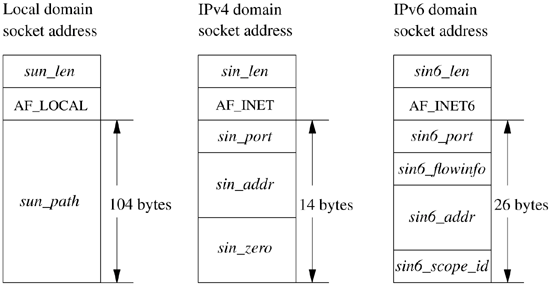
\includegraphics{images/sock_struct.png}}
	\caption{Δομές διευθυνσιοδότησης για sockets \href{http://www.ico.aha.ru/h/The\_Design\_and\_Implementation\_of\_the\_FreeBSD\_Operating\_System/ch11lev1sec4.htm}{πηγή}}
	\label{sock_struct}
\end{figure*} 




\subsubsection*{bind}
\begin{lstlisting}[language=C,breaklines=true, frame=none, backgroundcolor=\color{lightgray}, basicstyle=\footnotesize\ttfamily]
#include <sys/types.h>          
#include <sys/socket.h>
int bind(int sockfd, const struct sockaddr *addr, socklen_t addrlen)
\end{lstlisting}

Για τη χρήση των κλήσεων των sockets πρέπει να χρησιμοποιήσουμε το   <sys/socket.h>. Αν έχουμε να κάνουμε με UNIX domain sockets χρειάζεται το  <sys/un.h>, ενώ στην περίπτωση του internet domain απαιτείται η <netinet/in.h>. 

Η bind συνδέει ένα path ή μια διεύθυνση internet με ένα socket. Το πρώτο ορισμα (int sockfd) αναφέρεται στον περιγραφέα της υποδοχής και είναι
αυτό που μας επιστρέφει η socket(). Το δεύτερο όρισμα είναι μια δομή (struct) η οποία κρατάει τις πληροφορίες διευθυνσιοδότησης.

Το τρίτο όρισμα αναφέρεται στο μέγεθος (σε bytes) της δομής διεθυνσιοδότησης η οποία υποδυκνύεται από τη διεύθυνση μνήμης addr. Σε επιτυχία
η bind επιστρέφει 0 και σε αποτυχία -1. 

\subsection*{Συνδέοντας stream sockets}
Κατα την επικοινωνία δυο διεργασιών μέσω μιας υποδοχής, η μια διεργασία εκτελεί τον πάροχο υποδοχής και η άλλη τον πελάτη υποδοχής
(ακολουθώντας το μοντέλο client-server). Ο server «δεσμέυει» (binds) την υποδοχή στο συμφωνημένο path ή διεύθυνση δικτύου. Στη συνέχεια
μπλοκάρει την υποδοχή. Για μια SOCK\_STREAM υποδοχή ο server καλεί τη listen() στην οποία καθορίζονται πόσες αιτήσεις σύνδεσης θα
αποθηκεύονται στην ουρά.

\subsubsection*{listen}
\begin{lstlisting}[language=C,breaklines=true, frame=none, backgroundcolor=\color{lightgray}, basicstyle=\footnotesize\ttfamily]
#include <sys/types.h>          
#include <sys/socket.h>
 int listen(int sockfd, int backlog);
\end{lstlisting}


Η listen παίρνει 2 παραμέτρους: τον περιγραφέα υποδοχής (αυτόν που επιστρέφει η socket()) και το μέγεθος της ουράς (το μέγεθος των αιτήσεων
που θα περιμένουν ενόσω ο server χειρίζεται μια συγκεκριμένη σύνδεση).
Σε επιτυχία η listen επιστρέφει 0 και σε αποτυχία -1. 



Ο client ξεκινά μια σύνδεση με την υποδοχή του server καλώντας την connect().


\subsubsection*{connect}
\begin{lstlisting}[language=C,breaklines=true, frame=none, backgroundcolor=\color{lightgray}, basicstyle=\footnotesize\ttfamily]
#include <sys/types.h>          
#include <sys/socket.h>
int connect(int sockfd, const struct sockaddr *addr, socklen_t addrlen)
\end{lstlisting}


Στην περίπτωση του UNIX domain η connect είναι της μορφής:

\begin{lstlisting}[language=C,breaklines=true, basicstyle=\scriptsize\ttfamily]
struct sockaddr_un server;  
... 
connect (sd, (struct sockaddr *)&server, length);
\end{lstlisting}

ενώ στην περίπτωση του internet domain θα είναι:

\begin{lstlisting}[language=C,breaklines=true, basicstyle=\scriptsize\ttfamily]
struct sockaddr_in server; 
... 
connect (sd, (struct sockaddr *)&server, length);
\end{lstlisting}

Το πρώτο όρισμα και εδώ είναι ο περιγραφέας υποδοχής. Το δεύτερο όρισμα είναι η δομή η οποία κρατά πληροφορίες για τη διεύθυνση της
υποδοχής. Το τρίτο όρισμα αναφέρεται στο μέγεθος του δευτέρου ορίσματος.

Σε επιτυχία η connect επιστρέφει 0 και σε αποτυχία -1.

Στην περίπτωση του SOCK\_STREAM ο server καλεί την accept() ώστε να ολοκληρωθεί η σύνδεση.

\subsubsection*{accept}
\begin{lstlisting}[language=C,breaklines=true, frame=none, backgroundcolor=\color{lightgray}, basicstyle=\footnotesize\ttfamily]
#include <sys/types.h>          
#include <sys/socket.h>
int accept(int sockfd, struct sockaddr *addr, socklen_t *addrlen);
\end{lstlisting}

Η accept επιστρέφει έναν νέο περιγραφέα υποδοχής, ο οποίος είναι ενεργός μόνο για τη συγκεκριμένη σύνδεση (σχήμα \ref{socket_connect_ports}). Ένας server μπορεί να έχει
πολλαπλές SOCK\_STREAM συνδέσεις την ίδια στιγμή. Σε αποτυχία επιστρέφει -1. Σχετίζεται μόνο με connection-based socket types.  Χρειάζεται 3
παραμέτρους: η πρώτη είναι ο περιγραφέας της υποδοχής, το δεύτερο είναι η δομή για τη διεύθυνση της υποδοχής (δείκτης σε δομή sockaddr) και
το τρίτο είναι το μέγεθος του δευτέρου ορίσματος.  

\begin{figure*} 
	\centering
	\scalebox{0.9}{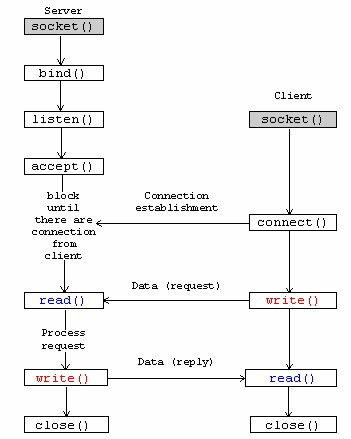
\includegraphics{images/sock-conn.png}}
	\caption{Επικοινωνία με υποδοχές (SOCK\_STREAM)}
\end{figure*} 


\begin{figure*} 
	\centering	\scalebox{0.5}{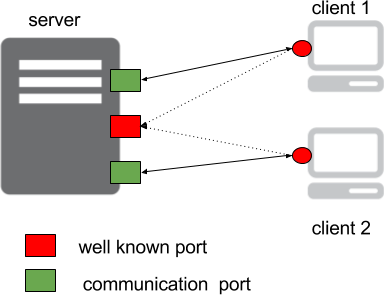
\includegraphics{images/socket_connect_ports.png}}
	\caption{Όταν συνδέεται ένας client}
	\label{socket_connect_ports}
\end{figure*} 


\subsection*{Μεταφορά δεδομένων και κλείσιμο}
Υπάρχουν πολλοί τρόποι για αποστολή και λήψη δεδομένων από ένα SOCK\_STREAM socket. Αυτές είναι οι write(), read(), send() και recv(). Οι
δυο τελεταίες είναι παρόμοιες με τις write() και read() απλά έχουν επιπρόσθετες παραμέτρους.

\subsubsection*{send}
\begin{lstlisting}[language=C,breaklines=true, frame=none, backgroundcolor=\color{lightgray}, basicstyle=\footnotesize\ttfamily]
#include <sys/types.h>          
#include <sys/socket.h>
ssize_t send(int sockfd, const void *buf, size_t len, int flags);
\end{lstlisting}

\subsubsection*{recv}
\begin{lstlisting}[language=C,breaklines=true, frame=none, backgroundcolor=\color{lightgray}, basicstyle=\footnotesize\ttfamily]
#include <sys/types.h>          
#include <sys/socket.h>
ssize_t recv(int sockfd, void *buf, size_t len, int flags);
\end{lstlisting}

Η επιπλέον παράμετρος flags \footnote{\href{http://www.gnu.org/software/libc/manual/html\_node/Out\_002dof\_002dBand-Data.html}{out-of-bound data}} μπορεί να είναι συνδυασμός των παρακάτω flags ή και τίποτα από αυτά:

\begin{table}[h]
	\begin{tabularx}{\columnwidth}{l|X}
		\textbf{MSG\_OOB} &  Στείλε out-of-band δεδομένα. Μόνο τα SOCK\_STREAM sockets τα οποία έχουν δημιουργηθεί στο internet domain τα
		υποστηρίζουν \\
		\textbf{MSG\_DONTROUTE} & Αφορά τη διάρκεια και χρησιμοποιείται μόνο από διαγνωστικά προγράμματα \\
		\textbf{MSG\_PEEK} & Τα δεδομένα παραμένουν στην υποδοχή, ώστε μια επόμενη recv() να τα ξαναδεί
	\end{tabularx}  
	\caption{Flags των send() και recv()}
\end{table}

Ένα stream socket καταστρέφεται καλώντας την close() και δίνοντας σαν παράμετρο τον περιγραφέα υποδοχής.
Μπορείτε να δείτε το \href{https://goo.gl/Ryx7Ku}{https://goo.gl/Ryx7Ku} για μια σύνοψη όλων των κλήσεων. 'Οταν τρέχετε εφαρμογές οι οποίες επικοινωνούν με sockets μπορείτε να χρησιμοποιείτε την εντολή netstat για να βλέπετε πληροφορίες που αφορούν τα  πρωτόκολλα επικοινωνίας, τα ports και την κατάσταση στης σύνδεσης. Μια συνηθισμένη χρήση της netstat είναι η
\begin{lstlisting}[language=C,breaklines=true, basicstyle=\scriptsize\ttfamily]
netstat -ant
\end{lstlisting}



\subsection*{Παράδειγμα: Stream Sockets in UNIX domain}

Δείτε το ζευγάρι server-client του κώδικα \ref{lab11-1-server} και \ref{lab11-1-client}, όπου παρουσιάζεται ένας echo server όπου ο server εμφανίζει τα μηνύματα του client.
Παρομοίως, το ζευγάρι server-client του κώδικα \ref{lab11-2-server} και \ref{lab11-2-client} εμφανίζεται ο client να στέλνει πολλαπλά μηνύματα στον server και αυτός να του απαντά με ό,τι έλαβε.

\lstinputlisting[float, language=C,breaklines=true,basicstyle=\scriptsize\ttfamily,caption={lab11\_1\_server.c:  Παράδειγμα server socket σε unix domain \#1}, label=lab11-1-server]{code/lab11_1_server.c}


\lstinputlisting[float, language=C,breaklines=true,basicstyle=\scriptsize\ttfamily,caption={lab11\_1\_client.c:Παράδειγμα client socket σε unix domain \#1}, label=lab11-1-client]{code/lab11_1_client.c}


\lstinputlisting[float, language=C,breaklines=true,basicstyle=\scriptsize\ttfamily,caption={lab11\_2\_server.c: Παράδειγμα server socket σε unix domain \#2}, label=lab11-2-server]{code/lab11_2_server.c}


\lstinputlisting[float, language=C,breaklines=true,basicstyle=\scriptsize\ttfamily,caption={lab11\_2\_client.c:Παράδειγμα client socket σε unix domain \#2}, label=lab11-2-client]{code/lab11_2_client.c}


\subsection*{Διάταξη των byte}
Όταν μεταβιβάζονται αλφαριθμητικά  μεταξύ των υπολογιστών ενός δικτύου, δεν δημιουργείται ποτέ πρόβλημα, επειδή κατά την επικοινωνία
διατηρείται πάντα η διάταξη των byte. Ωστόσο, κατά τη μεταβίβαση δυαδικών αριθμών μπορεί να υπάρξουν προβλήματα, αφού η διάταξη των byte σε
έναν αριθμό διαφέρει από υπολογιστή σε υπολογιστή
\footnote{\href{http://en.wikipedia.org/wiki/Endianness}{http://en.wikipedia.org/wiki/Endianness}} (Σχήμα \ref{endianess}. The Intel x86 family uses the little endian format).


\begin{figure} 
	\centering
	\scalebox{0.8}{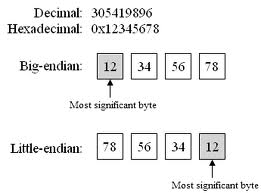
\includegraphics{images/endianess.jpg}}
	\caption{Διάταξη μικρού και μεγάλου άκρου}
	\label{endianess}
\end{figure}



Η λύση είναι η αποστολή δυαδικών αριθμών με μια προσυμφωνημένη δικτυακή διάταξη. Έτσι όλοι οι αποστολείς θα πρέπει να μετατρέψουν τη
διάταξη των byte από την τοπικη της μορφή στη δικτυακή, και όλοι οι παραλήπτες να μετατρέπουν τη δικτυακή μορφή στην τοπική. Αυτό γίνεται
μόνο για δεδομένα τα οποία δεν είναι ήδη δομημένα με κάποιον άλλο τρόπο (π.χ. μια εικόνα jpeg θα τη στείλετε ως έχει).

Συνήθως δε χρειάζεται να γνωρίζετε ούτε την τοπική ούτε τη δικτυακή διάταξη byte, αφού υπάρχει τυποποιημένο σύνολο συναρτήσεων «μετάφρασης»
οι οποίες πραγματοποιούν τις μετατροπές για ακεραίους των 16 και 32 bit. 


\begin{table}[h]
	\begin{tabularx}{\columnwidth}{l|X}
		\textbf{htons} & Μετατροπή 16bit τιμής από τοπική σε δικτυακή διάταξη byte (port number) \\
		\textbf{htonl} & Μετατροπή 32bit τιμής από τοπική σε δικτυακή διάταξη byte (ip address) \\
		\textbf{ntohs} & Μετατροπή 16bit τιμής από δικτυακή σε τοπική διάταξη byte (read a port number from sockaddr)\\
		\textbf{ntohl} & Μετατροπή 32bit τιμής από δικτυακή σε τοπική διάταξη byte  (read ip from sockaddr) \\
	\end{tabularx}  
	\caption{Συναρτήσεις «μετάφρασης»}
\end{table}



\subsection*{inet\_ntop}

Σύνταξη: inet\_ntop (numeric to presentation, binary value (socket address structure) to ASCII string (dotted-decimal string))
\begin{lstlisting}[language=C,breaklines=true, basicstyle=\scriptsize\ttfamily]
#include <arpa/inet.h>
const char *inet_ntop(int af, const void *src, char *dst, socklen_t size);
\end{lstlisting}

Η κλήση αυτή μετατρέπει τη δομή διεύθυνσης δικτύου \emph{src} η οποία είναι της \emph{af} address family σε ένα string. 
Το επιστρεφόμενο string αντιγράφεται σε ένα buffer που δείχνει ο \emph{dst} pointer, ο οποίος πρέπει να είναι ένας no-null pointer.
To \emph{size} είναι το μέγεθος των επιστρεφόμενων δεδομένων. Για το λόγο αυτό (size) υπάρχουν οι ακόλουθες δηλώσεις\footnote{Πρέπει να κάνουμε include τη <netinet/in.h>}:


{\color{red}\textbf{Σημείωση:} Για να τρέξουμε τον κώδικα του εργαστηρίου σε περιβάλλον Solaris, θα πρέπει να βάλουμε στο gcc τις παραμέτρους -lsocket και -lnsl}


\begin{lstlisting}[language=C,breaklines=true, basicstyle=\scriptsize\ttfamily]
#define INET_ADDRSTRLEN 16 /* for IPv4 dotted-decimal*/
#define INET6_ADDRSTRLEN 32 /* for IPv6 hex string*/
\end{lstlisting}

Υπάρχει και η αντίστροφη μετατροπή, από presentation to numeric (inet\_pton). Μετατρέπει μια IP διεύθυνση από string σε network byte order. (Σχήμα \ref{pton})

\begin{lstlisting}[language=C,breaklines=true, basicstyle=\scriptsize\ttfamily]
#include <arpa/inet.h>
int inet_pton(int af,const char *src,void *dst); 
\end{lstlisting}



\begin{figure}[!h]
	\centering
	%\scalebox{0.2}{\includegraphics{unix-tree.eps}}
	%\resizebox{\linewidth}{!}{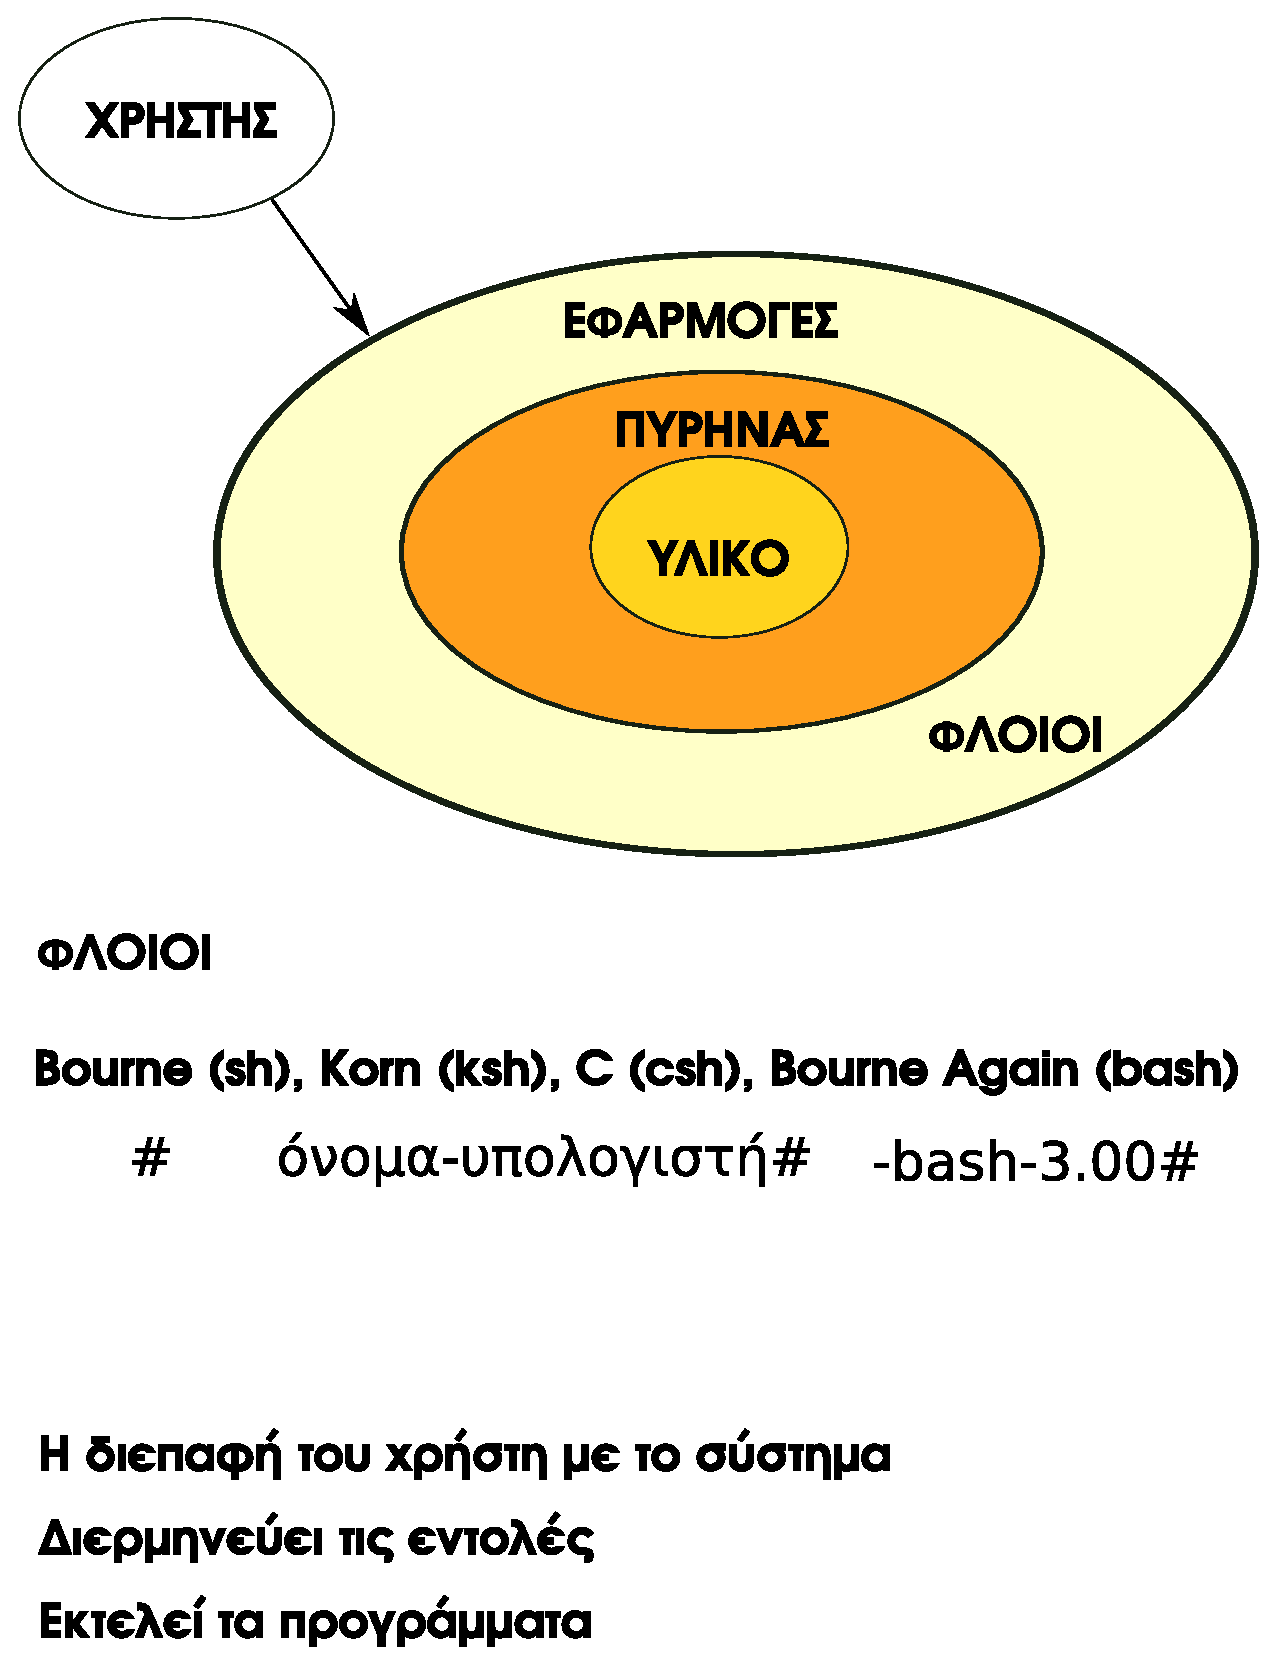
\includegraphics{shells.eps}}
	\scalebox{0.8}{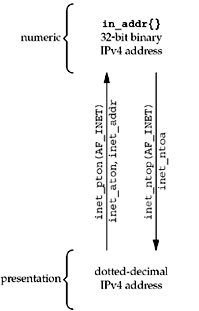
\includegraphics{images/pton.png}}
	\caption{Συναρτήσεις μετατροπής διευθύνσεων network byte order σε presentation}
	\label{pton}
\end{figure} 

\begin{figure*}[!h]
	\centering
	%\scalebox{0.2}{\includegraphics{unix-tree.eps}}
	%\resizebox{\linewidth}{!}{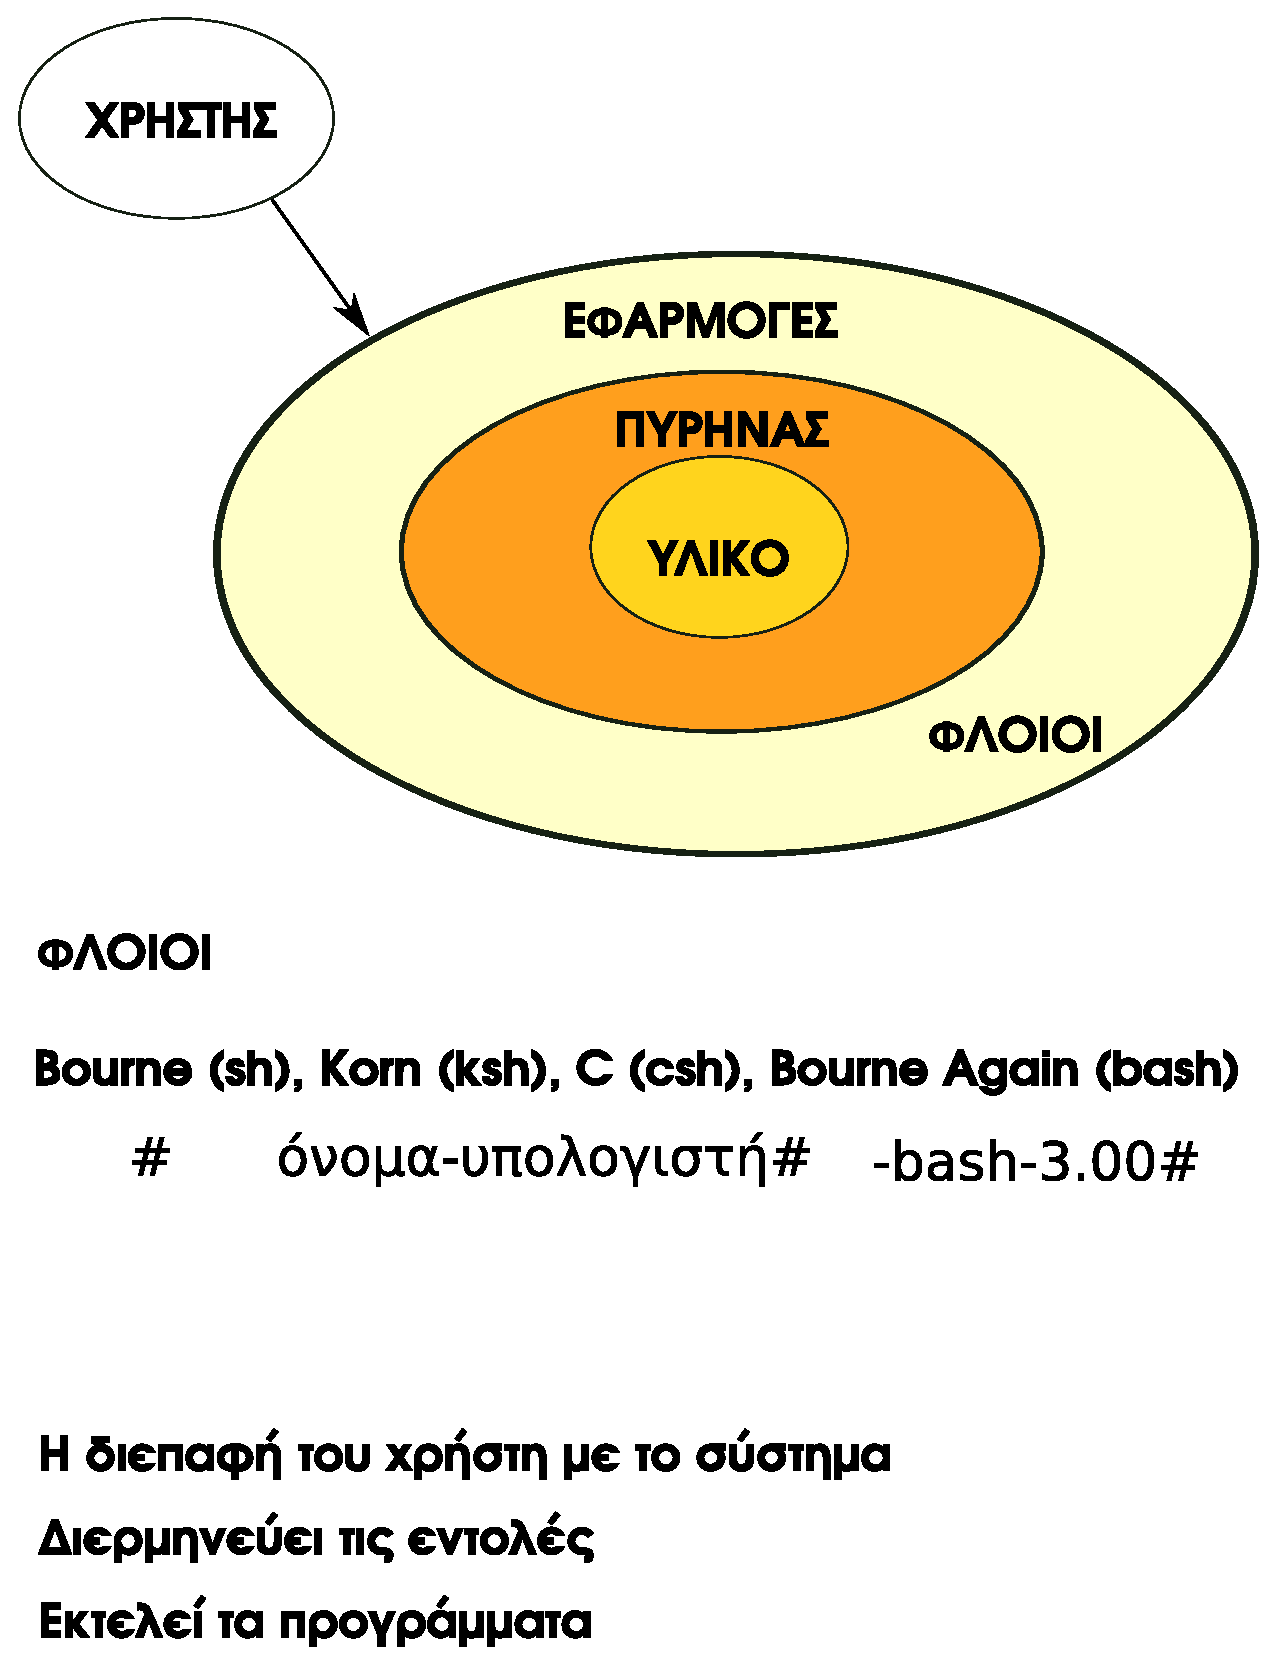
\includegraphics{shells.eps}}
	\scalebox{0.6}{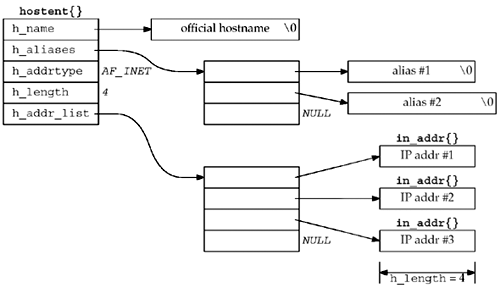
\includegraphics{images/hostent.png}}
	\caption{Η δομή hostent}
	\label{hostent}
\end{figure*} 



\lstinputlisting[float, language=C,breaklines=true,basicstyle=\scriptsize\ttfamily,caption={lab11\_3.c:Παράδειγμα μετατροπών network byte order σε presentation και αντίστροφα}, label=lab11-3]{code/lab11_3.c}

%\lstinputlisting[language=C, caption={lab11\_3.c:Παράδειγμα μετατροπών network byte order σε presentation και αντίστροφα}]{code/lab11_3.c}


\subsection*{Δομή hostent}

Σε πολλές περιπτώσεις μπορεί να γνωρίζουμε το όνομα (hostname) ενός υπολογιστή, παρά τη δικτυακή του διεύθυνση (ip address). Για να μπορούμε να πάρουμε την ip address από ένα hostname, είναι να χρησιμοποιήσουμε την gethostbyname.

Στο σχήμα \ref{hostent} θα δείτε τη δομή hostent. Για να αναζητήσουμε ένα όνομα υπολογιστή στο διαδίκτυο, χρησιμοποιούμε την κλήση
gethostbyname δέχεται σαν παράμετρο το hostname και μας επιστρέφει έναν δείκτη σε αυτή τη δομή, η οποία περιέχει τις IP διευθύνσεις για τον υπολογιστή αυτό.
Συγκεκριμένα:

\begin{lstlisting}[language=C,breaklines=true, basicstyle=\scriptsize\ttfamily]
struct hostent {
	char  *h_name;            /* official name of host */
	char **h_aliases;         /* alias list */
	int    h_addrtype;        /* host address type */
	int    h_length;          /* length of address */
	char **h_addr_list;       /* list of addresses */
}
\end{lstlisting}




\lstinputlisting[float, language=C,breaklines=true,basicstyle=\scriptsize\ttfamily,caption={lab11\_4.c:Παράδειγμα gethostbyname}, label=lab11-4]{code/lab11_4.c}



%\lstinputlisting[language=C, caption={lab11\_4.c:Παράδειγμα gethostbyname}]{code/lab11_4.c}

\subsection*{INADDR\_ANY}
Χρησιμοποιούμε τη σταθερά INADDR\_ANY, ούτως ώστε να πάρει αυτόματα τη δικτυακή διεύθυνση του μηχανήματος. Τη χρησιμοποιούμε για να κάνουμε bind σε όλα τα network interfaces (π.χ. όταν είμαστε συνδεδεμένοι και με wifi και με ethernet, θα έχουμε 2 network interfaces με 2 ip addresses).
Με αυτόν τον τρόπο αφήνουμε το λειτουργικό να επιλέξει όποια θέλει.




\subsection*{Παράδειγμα: Stream Sockets in internet domain}


Ο κώδικας \ref{lab11-5-server} παρουσιάζει έναν stream socket server, βασισμένο σε TCP. Ο κώδικας \ref{lab11-5-client} παρουσιάζει τον αντίστοιχο client. Για να εκτελστεί ο server χρειάζεται μια παράμετρο που είναι η port στην οποία θα ακούει. Αντίστοιχα ο client \footnote{Η δομή hostent έχει και το εξής:\\  \#define h\_addr  h\_addr\_list[0]  /* for backward compatibility */} χρειάζεται δυο παραμέτρους: την ip διεύθυνση του server και την port.

\lstinputlisting[float, language=C,breaklines=true,basicstyle=\scriptsize\ttfamily,caption={lab11\_5\_server.c:Παράδειγμα server socket σε network domain}, label=lab11-5-server]{code/lab11_5_server.c}

%\lstinputlisting[language=C, caption={lab11\_5\_server.c:Παράδειγμα server socket σε network domain}]{code/lab11_5_server.c}


\lstinputlisting[float, language=C,breaklines=true,basicstyle=\scriptsize\ttfamily,caption={lab11\_5\_client.c:Παράδειγμα client socket σε network domain}, label=lab11-5-client]{code/lab11_5_client.c}




%\lstinputlisting[language=C, caption={lab11\_5\_client.c:Παράδειγμα client socket σε network domain}]{code/lab11_5_client.c}



\subsection*{Datagram sockets}
Ένα datagram δεν απαιτεί την εγκαθίδρυση σύνδεσης. Κάθε μήνυμα κουβαλά τη διεύθυνση προορισμού του. Αν μια συγκεκριμένη τοπική διεύθυνση
χρειάζεται, τότε μια κληση bind() πρέπει να προηγηθεί της μεταφοράς δεδομένων. Τα δεδομένα αποστέλλονται και λαμβάνονται χρησιμοποιώντας της
κλήσεις sendto() ή sendmsg(). Η sendto() είναι σαν την send() με τη διεύθυνση προορισμού να καθορίζεται. Για να λάβουμε datagram socket
μηνύματα χρησιμοποιούμε την recvfrom() ή την recvmsg(). Ενώ η recv() απαιτεί έναν buffer για τα αφιχθέντα δεδομένα, η recvfrom() απαιτεί δύο
buffers, έναν για το εισερχόμενο μήνυμα και ένα για τη λήψη της διεύθυνσης αποστολέα. 

Τα datagram sockets μπορούν επίσης να χρησιμοποιήσουν την connect() ώστε να συνδέσουν την υποδοχή σε συγκεκριμένη υποδοχή προορισμού. Όταν
αυτό συμβαίνει, χρησιμοποιούνται οι send() και recv() για την αποστολή/παραλαβή δεδομένων. Οι accept() και listen() δεν χρησιμοποιούνται
από τα datagram sockets.



\lstinputlisting[float, language=C,breaklines=true,basicstyle=\scriptsize\ttfamily,caption={lab11\_6\_server.c:Παράδειγμα UDP server σε network domain}, label=lab11-6-server]{code/lab11_6_server.c}

%\lstinputlisting[language=C, caption={lab11\_6\_server.c:Παράδειγμα UDP server σε network domain}]{code/lab11_6_server.c}


\lstinputlisting[float, language=C,breaklines=true,basicstyle=\scriptsize\ttfamily,caption={lab11\_6\_client.c:Παράδειγμα UDP client σε network domain}, label=lab11-6-server]{code/lab11_6_client.c}


%\lstinputlisting[language=C, caption={lab11\_6\_client.c:Παράδειγμα UDP client σε network domain}]{code/lab11_6_client.c}


Περισσότερες πληροφορίες μπορείτε να βρείτε στα \cite{NetSockets,UnixSockets, SocketsTutorial, Beej, Endianness, OutOfBound, SocketsIntro, TCPConTerm, SockAddrStruct, ReadSock, Sockets} και στο βιβλίο \cite{stevens2004unix}.


